\documentclass{article}

\usepackage[utf8]{inputenc}     % pdfLaTeX
\usepackage[T1]{fontenc}

\usepackage{amsthm}
\usepackage{amsmath}
\usepackage{tikz}
\usetikzlibrary{arrows.meta, positioning}
\usepackage{graphicx} % Required for inserting images
% who the fuck puts that comment there lmao
% most internet-copied thing ever
% lol
% we are NOT releasing this without checking these comments first :sob: 
%lowk just copying it from another overleaf default project lmao
%anyways gonna start working on it now
\theoremstyle{definition}
\newtheorem{definition}{Definition}[section]

\newtheorem*{remark}{Remark}

\theoremstyle{definition}
\newtheorem{example}{Example}

\title{Graph Theory}
\author{Simon László}
\date{Last updated: March 2026}

\begin{document}

\maketitle

\section{Graphs}
\begin{definition}[Graphs]
A graph is made up of vertices and edges. An edge either connects two vertices or one vertex to itself.
\end{definition}

\begin{remark}
We will show 3 ways to represent data.
\begin{enumerate}
\item Whatever the fuck this is called form: \\ \\
\begin{matrix}
A & B & C & D & E\\
AB & AC & BC & DE & EE
\end{matrix}

\item Graph form: \\ \\
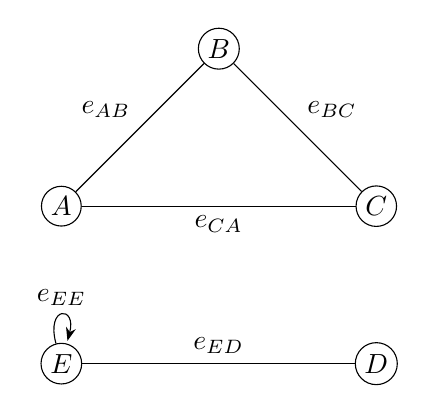
\begin{tikzpicture}[
    vertex/.style={circle, draw, inner sep=1.5pt},
    >=Stealth]

% Top part A B C
\node[vertex] (A) at (0,0) {$A$};
\node[vertex] (C) at (4,0) {$C$};
\node[vertex] (B) at (2,2) {$B$};
\draw[-] (A) -- node[above left] {$e_{AB}$} (B);
\draw[-] (B) -- node[above right] {$e_{BC}$} (C);
\draw[-] (A) -- node[below] {$e_{CA}$} (C);

% Bottom part D E
\node[vertex] (E) at (0,-2) {$E$};
\node[vertex] (D) at (4,-2) {$D$};
\draw[-] (E) -- node[above] {$e_{ED}$} (D);
\draw[-] (E) edge[loop above] node {$e_{EE}$} ();
\end{tikzpicture}

% I'm going to end your lineage with this shit
%thank chatgpt lmao
% fahhhh LMAO
%reading through these comments later will be peak
% :sob:
%anyways what if we just left in the "Whatever the fuck this is called form"
% :sob: v2
%fahhhh 67th line btw (not anymore)
\item Matrix form: \\ \\
\begin{matrix}
 & A & B & C & D & E \\
 A & 0 & 1 & 1 & 0 & 0\\
 B & 1 & 0 & 1 & 0 & 0\\
 C & 1 & 1 & 0 & 0 & 0\\
 D & 0 & 0 & 0 & 0 & 1\\
 E & 0 & 0 & 0 & 1 & 1
\end{matrix}
\end{enumerate}
\end{remark}

\begin{definition}[Loop]
A loop is an edge which connects a vertex to itself.
\end{definition}
\begin{definition}[Parallel edges]
    Parallel edges are two or more edges which connect the same vertices.
\end{definition}
\begin{example} In graph form: \\
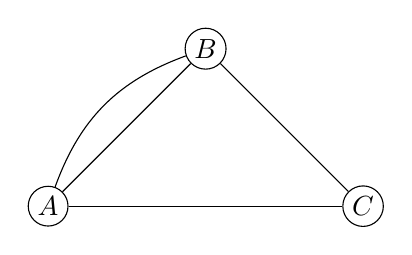
\begin{tikzpicture}[
    vertex/.style={circle, draw, inner sep=1.5pt},
    >=Stealth
]

\node[vertex] (A) at (0,0) {$A$};
\node[vertex] (C) at (4,0) {$C$};
\node[vertex] (B) at (2,2) {$B$};

\draw[-] (A) -- (B);
\draw[-] (B) -- (C);
\draw[-] (A) -- (C);

\draw[-, bend left=25] (A) to (B);

\end{tikzpicture}
\end{example}
\begin{definition}[Simple graph]
    A graph that contains no loops or parallel edges.
\end{definition}

\begin{definition}[Path]
    A path is a sequence of vertices and edges that connects a starting vertex to an ending vertex without repeating any vertices.
\end{definition}

\begin{definition}[Trail]
        A trail is a sequence of vertices and edges that connects a starting vertex to an ending vertex without repeating any edges.
\end{definition}

\begin{definition}[Walk]
    A walk is a finite, alternating sequence of vertices and edges, which defines traversal through a graph.
\end{definition}

\begin{definition}[Circuit]
    A circuit is a path that starts and ends at the same vertex, representing a closed loop.
\end{definition}

\begin{definition}[Hamiltonian Path]
    A Hamiltonian path is a path that contains all of the graph vertices.
\end{definition}

\begin{definition}[Hamiltonian Circuit]
    A Hamiltonian circuit is a circuit that contains all of the graph vertices.
\end{definition}

\begin{definition}[Euler Path]
    An Euler path is a trail that contains all of the graph edges.
\end{definition}

\begin{definition}[Euler Circuit]
    An Euler circuit is a circuit that contains all of the graph edges.
\end{definition}

\begin{definition}[Degree]
    The degree of a vertex is the amount of edges connected to the vertex. (A loop adds 2 to the degree of a vertex)
\end{definition}

\begin{definition}[Connected Graph]
    A connected graph is a graph in which there exists a path between any two given vertices.
\end{definition}

\begin{definition}[Component]
    A component of a graph is a maximal subgraph in which any two vertices are connected to each other by paths, and which is connected to no additional vertices in the graph.
\end{definition}


\end{document}